% This LaTeX was auto-generated from MATLAB code.
% To make changes, update the MATLAB code and export to LaTeX again.

\documentclass{article}

\usepackage[utf8]{inputenc}
\usepackage[T1]{fontenc}
\usepackage{lmodern}
\usepackage{graphicx}
\usepackage{color}
\usepackage{hyperref}
\usepackage{amsmath}
\usepackage{amsfonts}
\usepackage{epstopdf}
\usepackage[table]{xcolor}
\usepackage{matlab}
\usepackage[paperheight=795pt,paperwidth=614pt,top=72pt,bottom=72pt,right=72pt,left=72pt,heightrounded]{geometry}

\sloppy
\epstopdfsetup{outdir=./}
\graphicspath{ {./chemstability_final_es_media/} }

\begin{document}

\matlabtitle{Pruebas de Estabilidad Química}

\begin{par}
\begin{flushleft}
Las pruebas fueron realizadas en un período de 9 dias. 
\end{flushleft}
\end{par}

\begin{matlabcode}
clc; 
Time = [3 6 9]; % Tiempo de las pruebas
\end{matlabcode}


\matlabheading{Pérdida de peso de las pruebas de Estabilidad Ácida}

\matlabheadingthree{Ingreso de datos}

\begin{par}
\hfill \break
\end{par}

\begin{matlabcode}
z011 = [3.17 6.06 5.8]; %M1
z015 = [9.76 10.38 9]; %M2
z018 = [8.01 9.15 7.8]; %M2
z004a = [9.67 12.72 11.4]; %M3
z004b = [16.48 20.85 16.8]; %M3
Z030 = [9.7 9.8 10.40]; %M4
Z021 = [15.95 15.69 14.9]; %M5

\end{matlabcode}

\matlabheadingthree{Graficando los resultados}

\begin{par}
\hfill \break
\end{par}

\begin{matlabcode}
figure;
plot(Time,z011,'-o','DisplayName','M1');
hold on
plot(Time,z015,'-+','DisplayName','M2');
plot(Time,z004a,'-^','DisplayName','M3');
plot(Time,Z030,'--o','DisplayName','M4');
plot(Time,Z021,'-*','DisplayName','M5');

xlim([3 9]);
ylim([0 20]);
title('Pruebas de Estabilidad Ácida')
xlabel('Tiempo, dias')
ylabel('Pérdidad de peso, %')
legend 'show'

hold off
\end{matlabcode}
\begin{center}
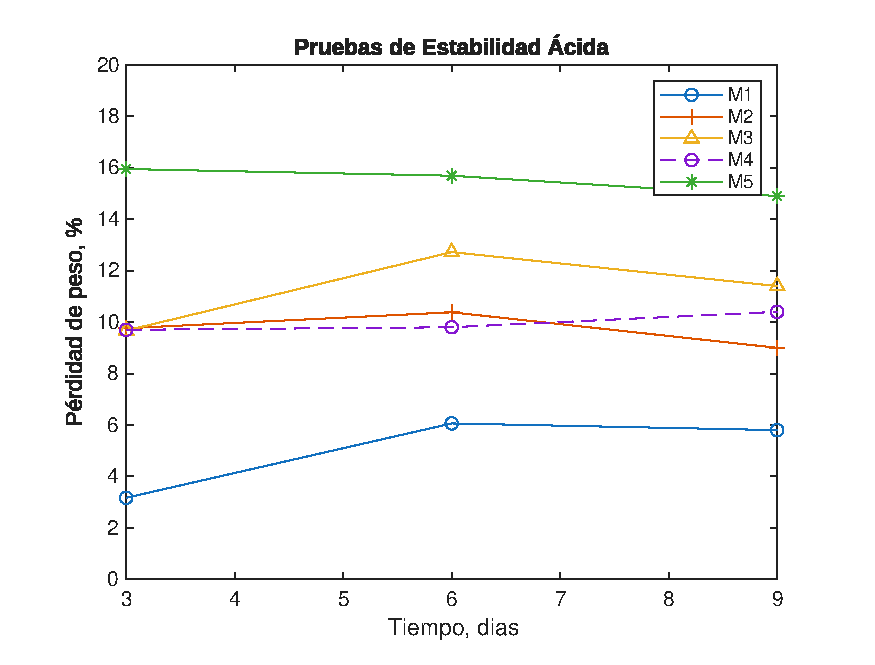
\includegraphics[width=\maxwidth{56.196688409433015em}]{est_ac.eps}
\end{center}


\matlabheading{Pérdida de peso de las pruebas de Estabilidad Alcalina}

\matlabheadingthree{Ingreso de datos}

\begin{par}
\hfill \break
\end{par}

\begin{matlabcode}
z022_alk = [45.44 55.13 44.6]; %M1
z020_alk = [-1.04 -1.21 -1.3]; %M2
z003_alk = [-1.46 -3.65 -5.9]; %M3
z009_alk = [-37.5 -39.39 -40.8]; %M4
z010b = [0.83 0.59 -0.8]; %M4
z014b = [-0.96 -0.68 0.5]; %M5
z021_alk = [-0.33 -0.48 -0.4]; %M5

\end{matlabcode}

\matlabheadingthree{Graficando los resultados}

\begin{par}
\hfill \break
\end{par}

\begin{matlabcode}
figure;
%plot(Time,z022_alk,'-o','DisplayName','M1');
hold on
plot(Time,z020_alk,'-+','DisplayName','M2');
plot(Time,z003_alk,'-^','DisplayName','M3');
plot(Time,z010b,'--o','DisplayName','M4');
plot(Time,z021_alk,'-*','DisplayName','M5');

xlim([3 9]);
ylim([-7 2]);
title('Pruebas de Estabilidad Alcalina')
xlabel('Tiempo, días')
ylabel('Pérdida de Peso, %')
legend 'show'

hold off
\end{matlabcode}
\begin{center}
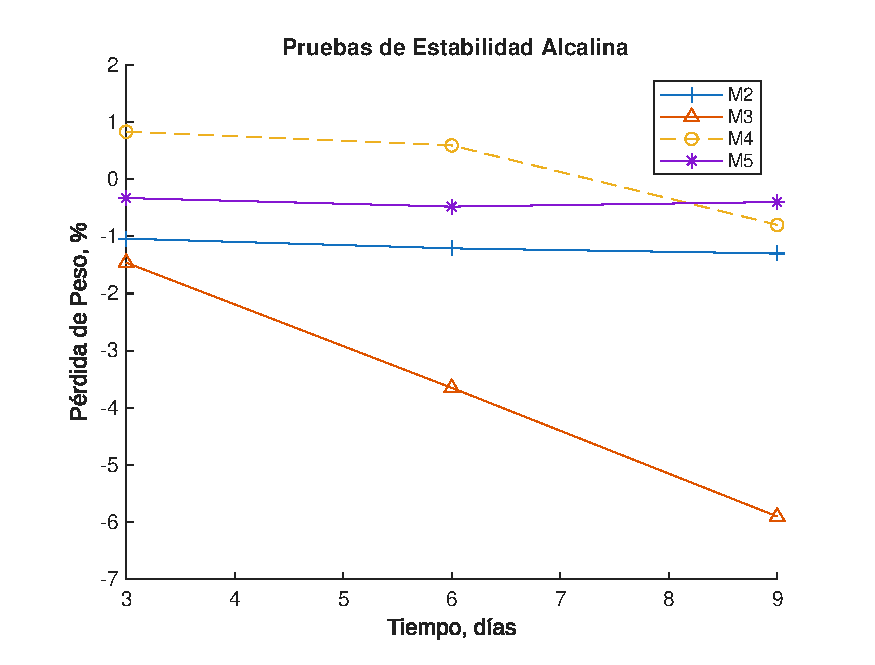
\includegraphics[width=\maxwidth{56.196688409433015em}]{est_alc.eps}
\end{center}

\end{document}
